\tdplotsetmaincoords{70}{20}
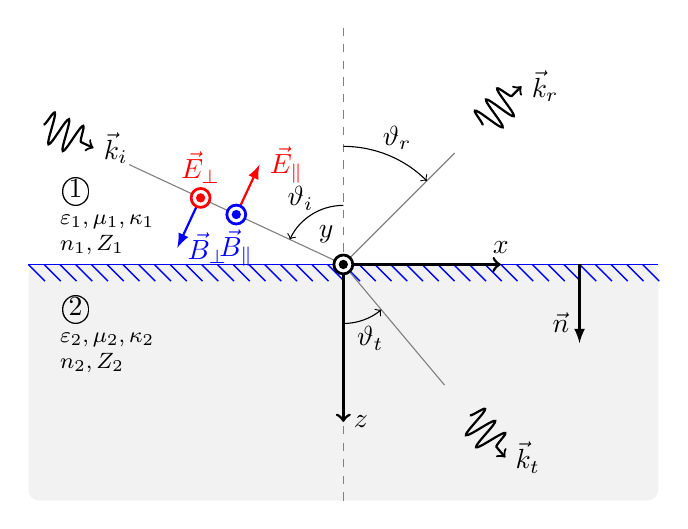
\begin{tikzpicture}[media/.style={font={\footnotesize}},wave/.style={decorate,decoration={snake,post length=1.4mm,amplitude=2mm,segment length=2mm},thick},
		interface/.style={
				% The border decoration is a path replacing decorator. 
				% For the interface style we want to draw the original path.
				% The postaction option is therefore used to ensure that the
				% border decoration is drawn *after* the original path.
				postaction={draw,decorate,decoration={border,angle=-45,
								amplitude=0.3cm,segment length=2mm}}},
	]
	% Round rectangle
	\fill[gray!10,rounded corners] (-4,-3) rectangle (4,0);
	% Interface
	\draw[blue,line width=.5pt,interface](-4,0)--(4,0);
	% Vertical dashed line
	\draw[dashed,gray](0,-3)--(0,3);
	% Coordinates system
	\draw(0,0.15)node[anchor=south east]{$y$};
	\draw[<->,line width=1pt] (2,0) node[above]{$x$}-|(0,-2) node[right]{$z$};
	% Incidence
	\draw[->,wave]
	(155:4.2cm)--(155:3.5cm)node[right]{$\vec{k}_i$};
	\draw[gray](0:0cm)--(155:3cm);
	\path (0,0)++(123:1cm)node{$\vartheta_i$};
	\draw[->](0,0.75)arc(90:155:.75cm);
	% EField
	\draw[red, -latex,thick](155:1.5)--+(65:0.7)node[right]{$\vec{E}_\parallel$};
	\filldraw[fill=white,draw=blue,line width=1pt](155:1.5)circle(.12cm) node[blue,below,yshift=-1.5]{$\vec{B}_\parallel$};
	\filldraw[fill=blue,draw=blue,line width=1pt](155:1.5)circle(.04cm);

	\draw[blue, -latex,thick](155:2)--+(245:0.7)node[right]{$\vec{B}_\perp$};
	\filldraw[fill=white,draw=red,line width=1pt](155:2)circle(.12cm) node[red,above,yshift=1.5]{$\vec{E}_\perp$};
	\filldraw[fill=red,draw=red,line width=1pt](155:2)circle(.04cm);

	% Transmission
	\draw[->,wave]
	(-50:2.5cm)--(-50:3.2cm)node[right]{$\vec{k}_t$};
	\draw[gray](0:0cm)--(-50:2cm);
	\path (0,0)++(-70:1cm)node{$\vartheta_t$};
	\draw[->] (0,-0.75) arc (-90:-50:.75cm);
	% Reflection
	\draw[->,wave]
	(45:2.5cm)--(45:3.2cm)node[right]{$\vec{k}_r$};
	\path (0,0)++(67:1.75cm) node{$\vartheta_r$};
	\draw[gray](0:0cm)--(45:2cm);
	\draw[->] (0,1.5)arc(90:45:1.5cm);
	% Media names
	\path[media] (-3,.6)  node[align=left]{{\normalsize\textcircled{1}\footnotesize}\\ $\varepsilon_1,\mu_1,\kappa_1$\\ $n_1, Z_1$}
	(-3,-.9) node[align=left]{{\normalsize\textcircled{2}\footnotesize}\\ $\varepsilon_2,\mu_2,\kappa_2$\\ $n_2, Z_2$};

	% $y$ axis
	\filldraw[fill=white,line width=1pt](0,0)circle(.12cm);
	\filldraw[fill=black,line width=1pt](0,0)circle(.04cm);
	% \draw[line width=.6pt] (0,0)
	%                       +(-135:.12cm) -- +(45:.12cm)
	%                       +(-45:.12cm) -- +(135:.12cm);

	\draw[thick,-latex] (3,0) -- (3,-1) node[anchor=south east]{$\vec{n}$};
\end{tikzpicture}